%!TEX program = lualatex
% SPDX-License-Identifier: CC-BY-SA-4.0
\documentclass[11pt]{article}

\usepackage{iftex}
\ifLuaTeX\else
  \PackageError{vintage-latex}{This example requires LuaLaTeX}
    {Run lualatex, not pdflatex or xelatex.}
\fi

\usepackage{fontspec}
\usepackage{xcolor}
\usepackage{geometry}
\usepackage[tracking=true,protrusion=false,expansion=false]{microtype}
\usepackage{tikz}
\usetikzlibrary{patterns.meta,calc}

\defaultfontfeatures{Renderer=HarfBuzz}
\setmainfont{EB Garamond}[Numbers={Lining,Proportional}]
\definecolor{sheetpaper}{HTML}{F5EDDF}
\definecolor{printerink}{HTML}{221E1A}
\pagecolor{sheetpaper}
\color{printerink}
\geometry{a4paper,top=16mm,bottom=16mm,left=20mm,right=20mm}
\pagestyle{empty}

\tikzset{
  outline/.style={draw=printerink,line width=.6pt,line join=round},
  thin outline/.style={draw=printerink,line width=.35pt},
  section/.style={pattern={Lines[angle=45,distance=2.4pt,line width=.28pt]},
                  pattern color=printerink},
  leader/.style={draw=printerink,line width=.28pt},
  numeral/.style={font=\footnotesize\itshape,inner sep=1pt,fill=sheetpaper}
}

% An engraved ball: outline clipped, then arcs of shadow drawn about a point
% displaced toward the light. Density increases away from the highlight.
\newcommand{\engravedball}[3]{% #1 centre, #2 radius in cm, #3 name
  \begin{scope}
    \clip #1 circle[radius=#2];
    \fill[sheetpaper] #1 circle[radius=#2];
    \foreach \k in {1,...,9} {
      \pgfmathsetmacro{\rr}{#2*(0.36+0.083*\k)}
      \pgfmathsetmacro{\lw}{0.16+0.022*\k}
      \draw[printerink,line width=\lw pt]
        ($#1+(-.32*#2,.32*#2)$) circle[radius=\rr];
    }
  \end{scope}
  \draw[outline] #1 circle[radius=#2];
}

\begin{document}

% Sheet heading in the style of the Patent Office plates.
\noindent
\makebox[\linewidth]{\footnotesize (No Model.)\hfill 2 Sheets---Sheet 1.}\par
\vspace{.9em}
\begin{center}
  {\large\textls[40]{J.\ HARGREAVE.}}\par
  \vspace{.35em}
  {\normalsize\textls[60]{CENTRIFUGAL GOVERNOR FOR STEAM ENGINES.}}\par
  \vspace{.35em}
  \footnotesize No.\ 214,731.\hspace{3em}Patented Apr.\ 22, 1879.
\end{center}

\vspace{2.2em}

\begin{center}
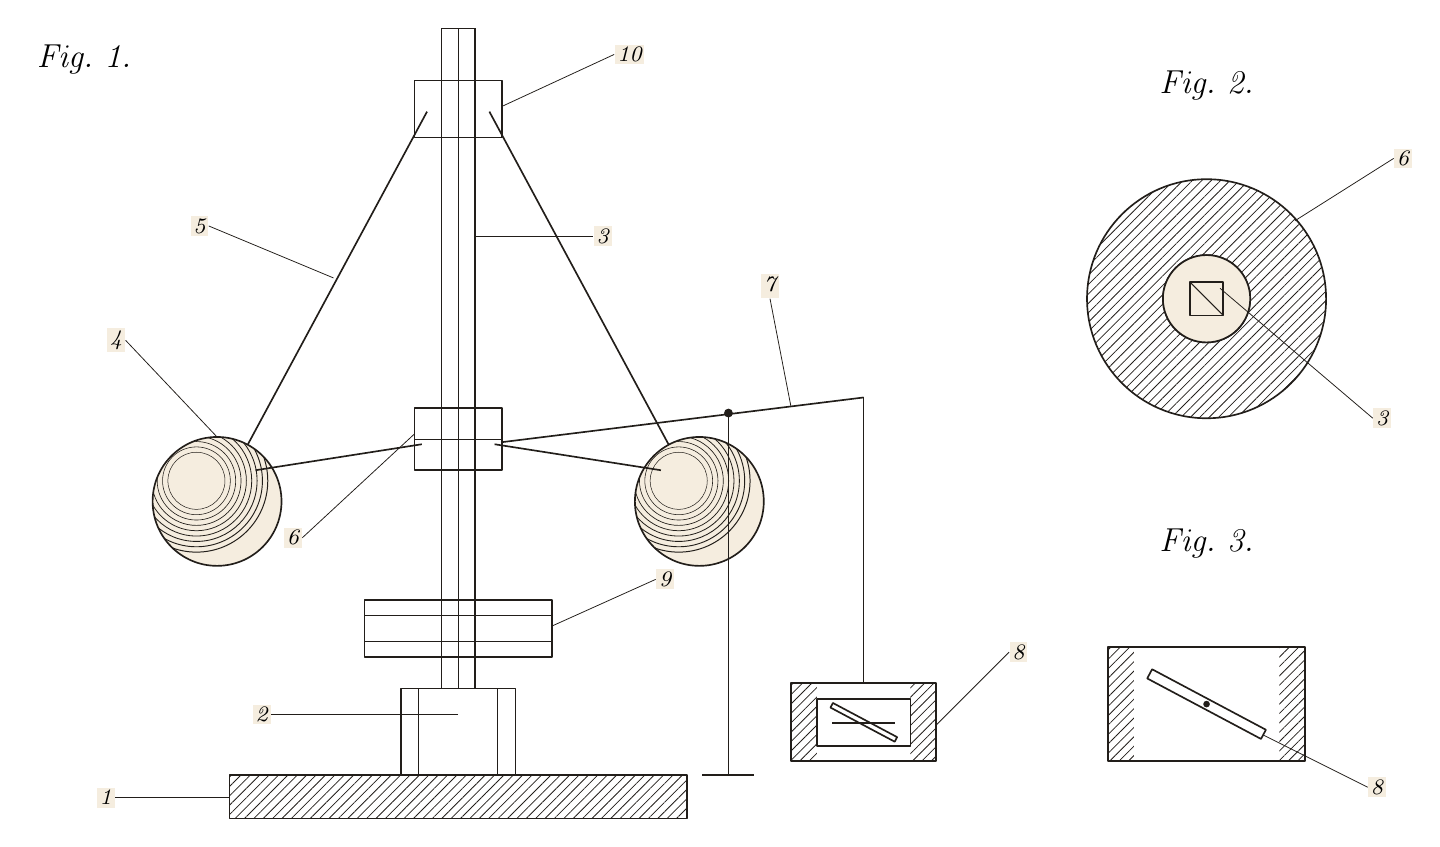
\begin{tikzpicture}[x=1.32cm,y=1.32cm]
  % ---- Fig. 1: elevation -------------------------------------------------
  \node[font=\large\itshape] at (-3.6,7.3) {Fig.\ 1.};

  % Base plate and bearing.
  \draw[outline] (-2.2,0) rectangle (2.2,.42);
  \path[section] (-2.2,0) rectangle (2.2,.42);
  \draw[outline] (-.55,.42) rectangle (.55,1.25);
  \draw[thin outline] (-.38,.42) -- (-.38,1.25) (.38,.42) -- (.38,1.25);

  % Spindle.
  \draw[outline] (-.16,1.25) -- (-.16,7.6) (.16,1.25) -- (.16,7.6);
  \draw[thin outline] (-.16,7.6) -- (.16,7.6);
  \draw[thin outline] (0,1.25) -- (0,7.6);

  % Collar at the top, from which the arms hang.
  \draw[outline] (-.42,6.55) rectangle (.42,7.1);

  % Arms and balls.
  \draw[outline] (-.3,6.8) -- (-2.05,3.55) (.3,6.8) -- (2.05,3.55);
  \engravedball{(-2.32,3.05)}{.62}{a}
  \engravedball{(2.32,3.05)}{.62}{b}

  % Sliding sleeve, with the lower links that raise it.
  \draw[outline] (-.42,3.35) rectangle (.42,3.95);
  \draw[thin outline] (-.42,3.65) -- (.42,3.65);
  \draw[outline] (-.35,3.6) -- (-1.95,3.35) (.35,3.6) -- (1.95,3.35);

  % Lever that carries the sleeve motion to the throttle valve.
  \draw[outline] (.42,3.62) -- (3.9,4.05);
  \draw[outline] (3.9,4.05) -- (3.9,1.3);
  \fill[printerink] (2.6,3.9) circle[radius=1.6pt];
  \draw[outline] (2.6,3.9) -- (2.6,.42);
  \draw[outline] (2.35,.42) -- (2.85,.42);

  % Throttle valve, shown in section on the steam pipe.
  \draw[outline] (3.2,.55) rectangle (4.6,1.3);
  \path[section] (3.2,.55) rectangle (3.45,1.3);
  \path[section] (4.35,.55) rectangle (4.6,1.3);
  \draw[outline] (3.45,.7) rectangle (4.35,1.15);
  \draw[outline] (3.6,.92) -- (4.2,.92);
  \draw[outline,rotate around={-28:(3.9,.92)}] (3.55,.9) rectangle (4.25,.95);

  % Driving pulley on the spindle.
  \draw[outline] (-.9,1.55) rectangle (.9,2.1);
  \draw[thin outline] (-.9,1.7) -- (.9,1.7) (-.9,1.95) -- (.9,1.95);

  % Reference numerals with plain leader lines and no arrowheads.
  \draw[leader] (-2.2,.2) -- (-3.3,.2);   \node[numeral,left] at (-3.3,.2) {1};
  \draw[leader] (0,1.0) -- (-1.8,1.0);    \node[numeral,left] at (-1.8,1.0) {2};
  \draw[leader] (.16,5.6) -- (1.3,5.6);   \node[numeral,right] at (1.3,5.6) {3};
  \draw[leader] (-2.32,3.67) -- (-3.2,4.6); \node[numeral,left] at (-3.2,4.6) {4};
  \draw[leader] (-1.2,5.2) -- (-2.4,5.7); \node[numeral,left] at (-2.4,5.7) {5};
  \draw[leader] (-.42,3.7) -- (-1.5,2.7); \node[numeral,left] at (-1.5,2.7) {6};
  \draw[leader] (3.2,3.97) -- (3.0,5.0);  \node[numeral,above] at (3.0,5.0) {7};
  \draw[leader] (4.6,.9) -- (5.3,1.6);    \node[numeral,right] at (5.3,1.6) {8};
  \draw[leader] (.9,1.85) -- (1.9,2.3);   \node[numeral,right] at (1.9,2.3) {9};
  \draw[leader] (.42,6.85) -- (1.5,7.35); \node[numeral,right] at (1.5,7.35) {10};

  % ---- Fig. 2: section through the sleeve ---------------------------------
  \begin{scope}[shift={(7.2,5.0)}]
    \node[font=\large\itshape] at (0,2.05) {Fig.\ 2.};
    \draw[outline] (0,0) circle[radius=1.15];
    \draw[outline] (0,0) circle[radius=.42];
    \path[section] (0,0) circle[radius=1.15];
    \fill[sheetpaper] (0,0) circle[radius=.42];
    \draw[outline] (0,0) circle[radius=.42];
    \fill[sheetpaper] (-.16,-.16) rectangle (.16,.16);
    \draw[outline] (-.16,-.16) rectangle (.16,.16);
    \draw[thin outline] (-.16,.16) -- (.16,-.16);
    \draw[leader] (.85,.75) -- (1.8,1.35); \node[numeral,right] at (1.8,1.35) {6};
    \draw[leader] (.13,.1) -- (1.6,-1.15);  \node[numeral,right] at (1.6,-1.15) {3};
  \end{scope}

  % ---- Fig. 3: detail of the valve disc -----------------------------------
  \begin{scope}[shift={(7.2,1.1)}]
    \node[font=\large\itshape] at (0,1.55) {Fig.\ 3.};
    \draw[outline] (-.95,-.55) rectangle (.95,.55);
    \path[section] (-.95,-.55) rectangle (-.7,.55);
    \path[section] (.7,-.55) rectangle (.95,.55);
    \draw[outline,rotate=-28] (-.62,-.05) rectangle (.62,.05);
    \fill[printerink] (0,0) circle[radius=1.2pt];
    \draw[leader] (.55,-.3) -- (1.55,-.8); \node[numeral,right] at (1.55,-.8) {8};
  \end{scope}
\end{tikzpicture}
\end{center}

\vfill
\noindent
\begin{minipage}[t]{.45\linewidth}
  \footnotesize\textls[70]{\textsc{Witnesses:}}\par
  \vspace{.9em}
  {\large\itshape Edw.\ Pellew}\par
  \vspace{.35em}
  {\large\itshape Thos.\ B.\ Carver}
\end{minipage}%
\hfill
\begin{minipage}[t]{.45\linewidth}
  \raggedleft
  \footnotesize\textls[70]{\textsc{Inventor:}}\par
  \vspace{.9em}
  {\large\itshape John Hargreave}\par
  \vspace{.35em}
  {\small\itshape by his Attorneys,}\par
  {\large\itshape Munn \& Co.}
\end{minipage}

\vspace{1.2em}
\footnotesize\noindent
Patent plates of the period share a small vocabulary: a sheet heading with
inventor, title, number, and date; italic figure numbers; parts identified by
numerals on plain leader lines; sections shown by hatching at forty-five
degrees; round parts modelled by curved line shading; and signature lines for
witnesses and inventor. All of it is ordinary text and TikZ paths.

\end{document}
